\documentclass[9pt]{beamer}

\mode<presentation> 
{ \usetheme[nat,dogma]{Frederiksberg} }

% \usepackage[danish]{babel}
\usepackage[latin1]{inputenc}
\usepackage{times}
\usepackage[T1]{fontenc}
\usepackage[english]{babel}
\usepackage{hyperref}
\usepackage{animate}
%\usepackage{multimedia}
\usepackage{francois-preamble}
\usepackage{multirow}
\usepackage{cancel}
\usepackage{multirow}
\usepackage{tikz} 
\usetikzlibrary{calc}
\usepackage{hhline}
\makeatletter
\newcommand\mathcircled[1]{%
  \mathpalette\@mathcircled{#1}%
}
\newcommand\@mathcircled[2]{%
  \tikz[baseline=(math.base)] \node[draw,circle,inner sep=1pt] (math) {$\m@th#1#2$};%
}
\makeatother

\newcommand{\tT}{\texttt{t}}
\newcommand{\tH}{\texttt{h}}

%\usepackage{movie15}

\newcommand{\cc}{{c\!\!,}}
\newcommand{\degr}[1]{{{#1}^\circ}}

\title{Vision and Image Processing:\\ Recalls on Probabilities and Statistcs}

\author[F.~Lauze] % (optional, use only with lots of authors)
{Fran{\c c}ois Lauze
}

\institute[DIKU] % (optional, but mostly needed)
{
  Department of Computer Science\\
  University of Copenhagen
}

\date[2017-18 B2] % (optional, should be abbreviation of conference name)
% {Research Presentation, Diku 2006}

\definecolor{gold}{rgb}{0.95,0.83,0.0}
\definecolor{orange}{rgb}{0.95,0.7,0.0}
% \definecolor{backblue}{rgb}{0.93,0.94,0.99}
\definecolor{backblue}{rgb}{0.95,0.94,0.99}
\setbeamercolor*{background canvas}{bg=backblue} 



\newcommand{\myemph}[1]{{\color{blue}{#1}}}
\newcommand{\intrg}[1]{\int_{{#1}=-\infty}^\infty}
\newcommand{\intRR}{\int_{-\infty}^\infty}

\AtBeginSection[]
{
  \begin{frame}<beamer>{Outline}
    \tableofcontents[currentsection,currentsubsection]
  \end{frame}
}

\begin{document}
\maketitle


%-------------------------------------------------------------------
%   Start slides
%-------------------------------------------------------------------




%----------------------------------------------



\begin{frame}
  \frametitle{Plan for today}
  \begin{itemize}
  \item Statistics. Observations, Means, Empirical Variance.
  \item Random Variables.
  \item Conditional Probabilities and Independence, Bayes Theorem
  \item Expectation, Variance, Moments.
  \item A Few Laws.
  \end{itemize}
\end{frame}

\begin{frame}\frametitle{Introduction}
  \begin{itemize}
  \item In real life, measurement process is not certain. 
  \item Repeating measurements often leads to small (or not that small) variations on results.
  \item Some ``average'' frequencies / range of measurements appear in general more often that others.
  \item Probabilities: quantification of uncertainty.
  \item Random variables: modelling of the measurements.
  \item Statistics: the practical / empirical observation part.
  \end{itemize}
\end{frame}


\section{Statistics}




\begin{frame}{Coin Example: Categorical Data}
  \begin{itemize}
  \item 20 coin flips:
    \begin{center}
    {\small
      \begin{tabular}[h]{|c|c|c|c|c|c|c|c|c|c|}\hline
        1 &   2 &   3 &  4  &   5 &   6 &   7 &   8 &   9 &  10 \\\hline
        \tT & \tT & \tT & \tH & \tT & \tT & \tH & \tH & \tT & \tT \\\hline
        11 &  12 &  13 &  14 &  15 &  16 &  17 &  18 &  19 &  20 \\\hline
        \tH & \tH & \tH & \tT & \tT & \tT & \tT & \tH & \tH & \tT\\\hline
      \end{tabular}
    }    
    \end{center}
  \item Fair coin?
  \item Frequency of heads: 8/20, tails: 12/20.
  \item Not 10/20 = 1/2, but not far away!
  \item Can I compute the mean result? Does it make sense?
  \item Here, categorical data: half tail, half head does not really make sense.
  \end{itemize}
\end{frame}


\begin{frame}
  \frametitle{Height Example: Numerical Data}
    \begin{itemize}
    \item 48 samples of heights of adult Scandinavian females (in cm).
      \begin{center}
        {\tiny
          \begin{tabular}[h]{|c|c|c|c|c|c|c|c|c|c|c|c|}
            \hline
            1 & 2 & 3 & 4 & 5 & 6 & 7 & 8 & 9 & 10 & 11 & 12\\\hline
            1.85 & 1.69 & 1.83 & 1.82 & 1.92 & 1.73 & 1.61 & 1.75 & 1.65 & 1.82 & 1.60 & 1.71
            \\\hhline{============}
            13 & 14 & 15 & 16 & 17 & 18 & 19 & 20 & 21 & 22 & 23 & 24\\\hline
            1.75 & 1.90 & 1.78 & 1.73 & 1.78 & 1.76 & 1.71 & 1.65 & 1.85 & 1.81 & 1.89 & 1.88
            \\\hhline{============}
            25 & 26 & 27 & 28 & 29 & 30 & 31 & 32 & 33 & 34 & 35 & 36\\\hline
            1.91 & 1.92 & 1.60 & 1.69 & 1.64 & 1.72 & 1.73 & 1.84 & 1.92 & 1.72 & 1.60 & 1.64
            \\\hhline{============}
            37 & 38 & 39 & 40 & 41 & 42 & 43 & 44 & 45 & 46 & 47 & 48\\\hline
            1.65 & 1.55 & 1.63 & 1.63 & 1.63 & 1.63 & 1.65 & 1.79 & 1.65 & 1.75 & 1.67 & 1.73
            \\\hline
          \end{tabular}
        }
      \end{center}
    \item Mean height? spread? repartition? Data is numerical here, this make sense.
    \item Max, Min, Mean, variance (average squared variation to the mean):
      \begin{align*}
        &\max h_i = 1.92,\quad\min h_i = 1.55,&\\
      &\bar{h} = \frac{1}{N}\sum_{i=1}^Nh_i = 1.74,\quad \sigma^2 =
      \frac{1}{N}\sum_{i=1}^n\left(h_i-\bar{h}\right)^2 = 0.010&
    \end{align*}
  \item Remember: standard deviation = $\sqrt{\text{variance}}$: $\sigma = 0.1$.
  \end{itemize}
\end{frame}

\begin{frame}
  \frametitle{Representation}
  \begin{center}{\tiny
      \setlength\tabcolsep{2pt}%
    \begin{tabular}[h]{|lcccccccccc|}
      \hline
      Range: & [1.55,1.58] & [1.59,1.62] & [1.63,1.66] & [1.67,1.69] & [1.70,1.73] & [1.74,1.77] & [1.78,1.80] & [1.81,1.84] & [1.85,1.88] & [1.89,1.92]\\
      \hline
      Count: & 1 & 4 & 11 & 3 & 8 & 4 & 4 & 4 & 3 & 6\\
      \hline
    \end{tabular}}
  \end{center}
  
  \begin{columns}
    \begin{column}{0.5\textwidth}
      \begin{center}
        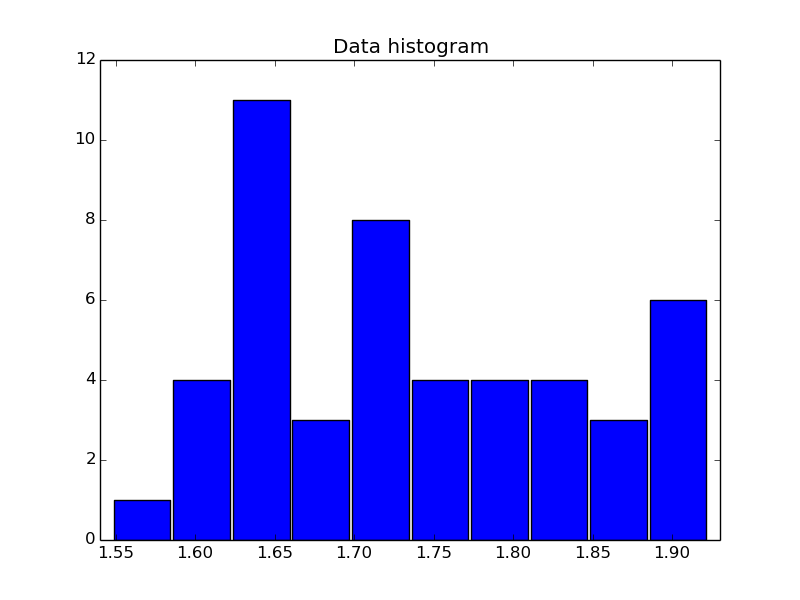
\includegraphics[width=0.9\textwidth]{FIGURES/dataheight_hist}
      \end{center}
    \end{column}
    \begin{column}{0.5\textwidth}
      \begin{itemize}
      \item Accumulate data in given ranges, a.k.a bins. 10 bins used here.
      \item Each bar displays amount of samples in a given range.
      \item Bin 3: range = [1.62, 1.66], 11 samples.
      \item Frequency that a sample is in range [1.63, 1.66]: 11/48.
      \end{itemize}
    \end{column}
  \end{columns} \pause
  \begin{itemize}
  \item Tempting to say that ``the probability that height is between 1.63 and 1.66 is 11/48''.
  \item With more samples maybe...
  \end{itemize}
\end{frame}


\begin{frame}{Image Histograms}
  \begin{center}
    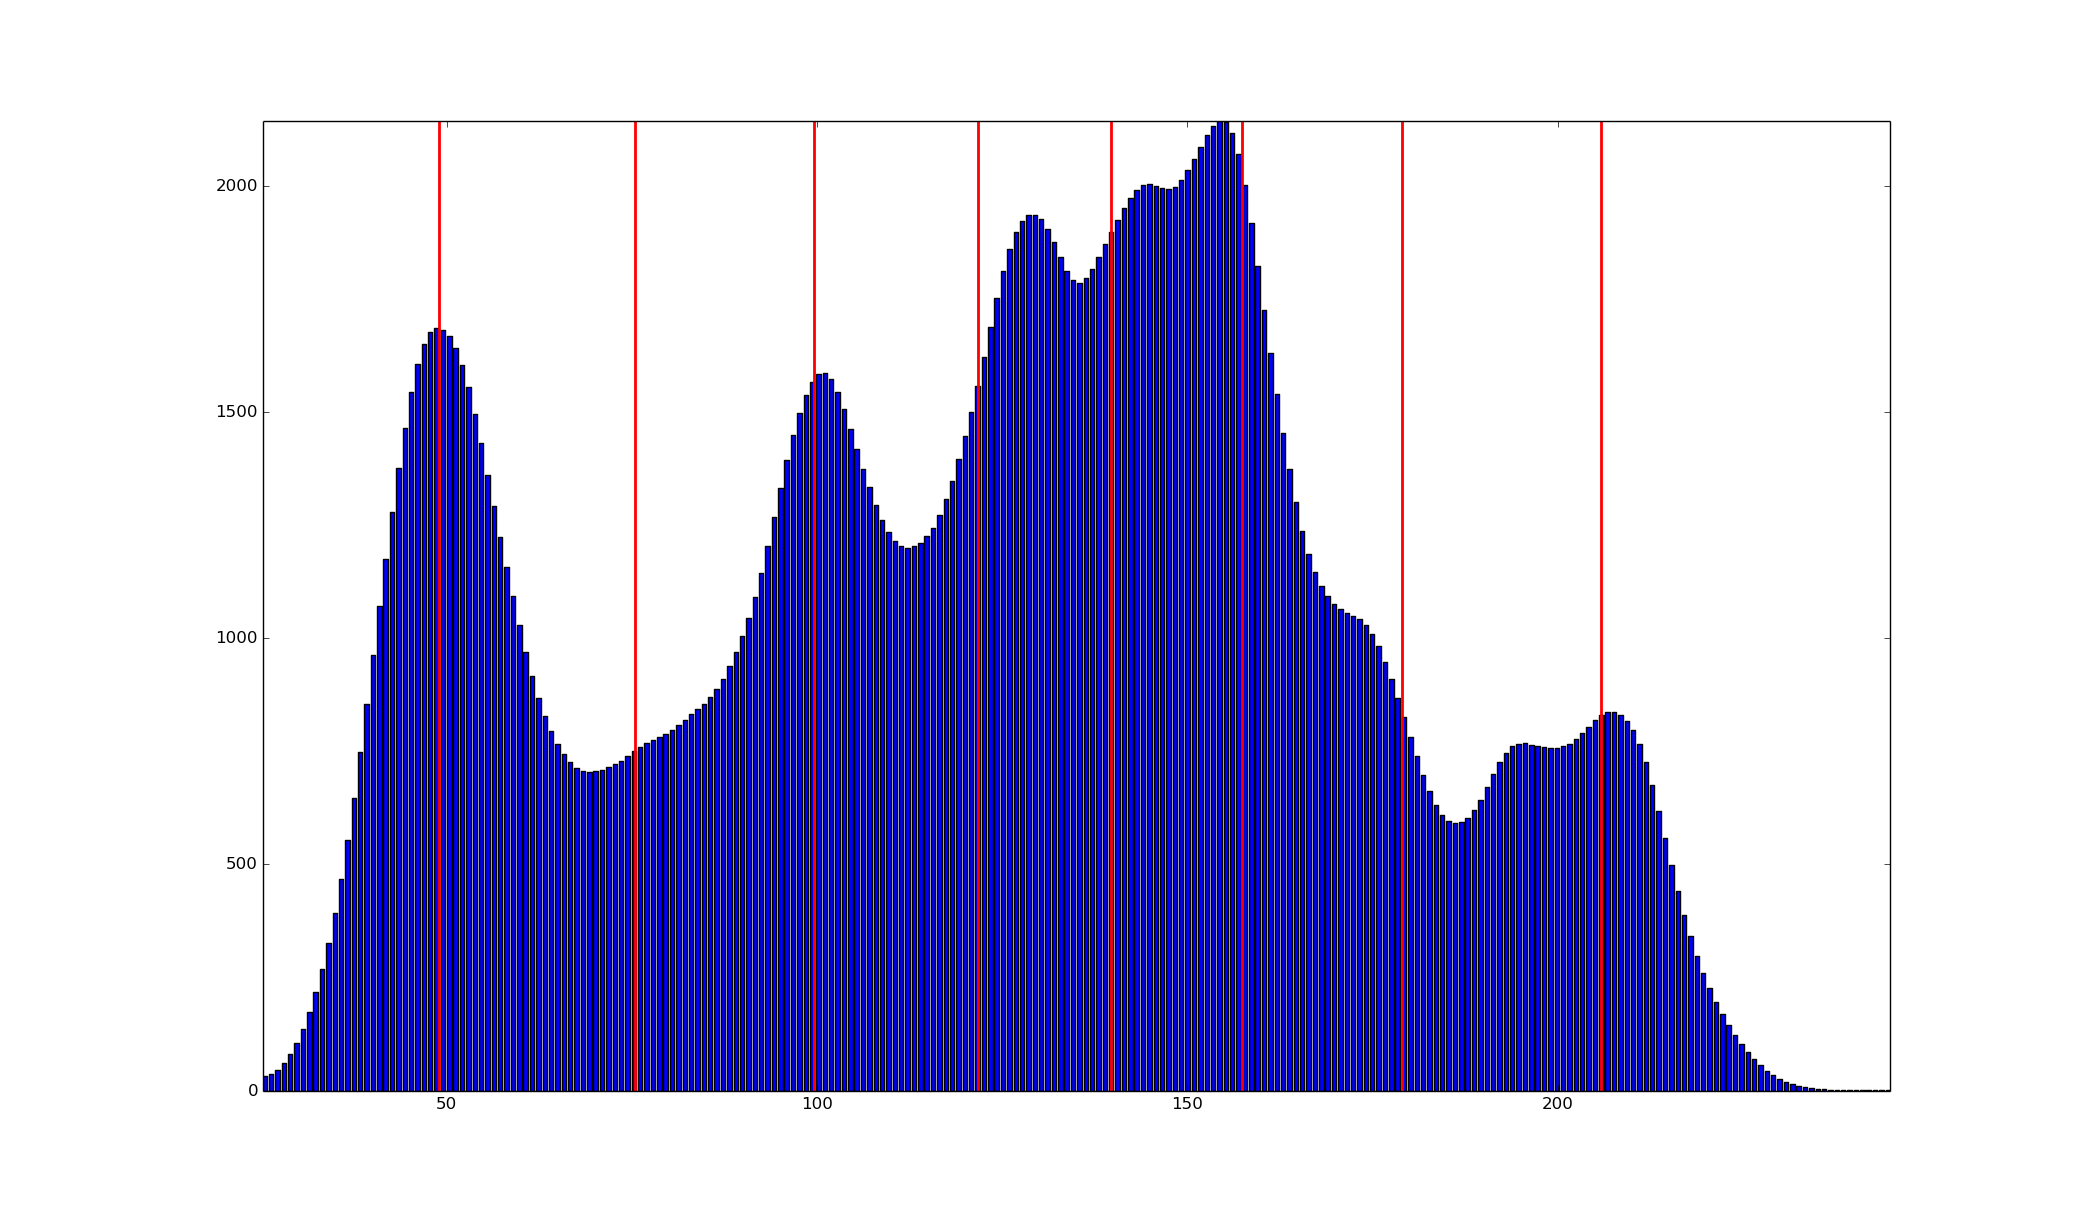
\includegraphics[width=0.9\textwidth]{FIGURES/lenahists}
  \end{center}
  \begin{itemize}
  \item Each bin represents a range of grey level values (here 100 bins).
  \item Each bin value represents a frequency of these grey values in image. 
  \end{itemize}
\end{frame}

\begin{frame}\frametitle{Recap}
  \begin{itemize}
  \item $N$ outcomes of an experiment, results in given categories $c_1,\dots, c_k$.
  \item Can talk of frequency of apparition of category $c_k$: 
    $$
    \frac{\text{number of outcomes in category }c_k}{\text{number of outcomes} = N}
    $$
  \item Can discuss of the largest represented category, smallest, mean category size\dots
  \item For numerical outcomes: grouping in ranges: histograms.
  \item Means, variances etc... make sense. Sample $h = (h_1,\dots,h_N)$:
    $$
    \bar{h} = \frac1N\sum_{i=1}^N h_i,\quad \sigma^2_h =  \frac1N\sum_{i=1}^N \left(h_i - \bar{h}\right)^2 = \left(\frac1N\sum_{i=1}^N h_i^2\right) - \bar{h}^2
    $$
  \end{itemize}
  
\end{frame}


\begin{frame}\frametitle{Bivariate Data}
  \begin{center}
    \begin{tabular}[h]{cc}
      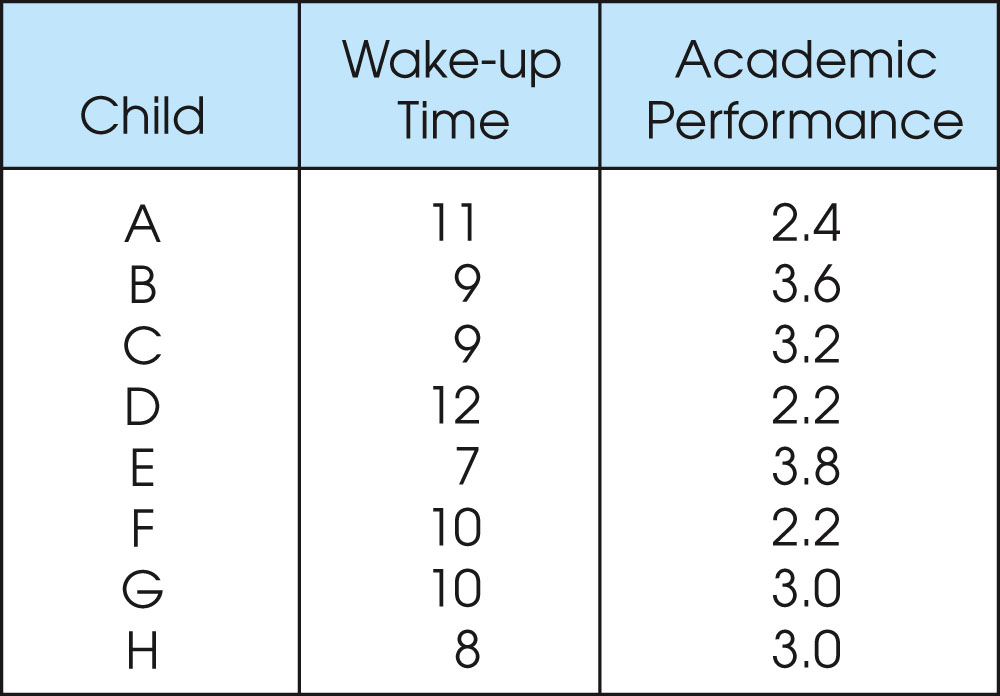
\includegraphics[width=0.45\textwidth]{FIGURES/wakeacademic1} & 
      \only<1>{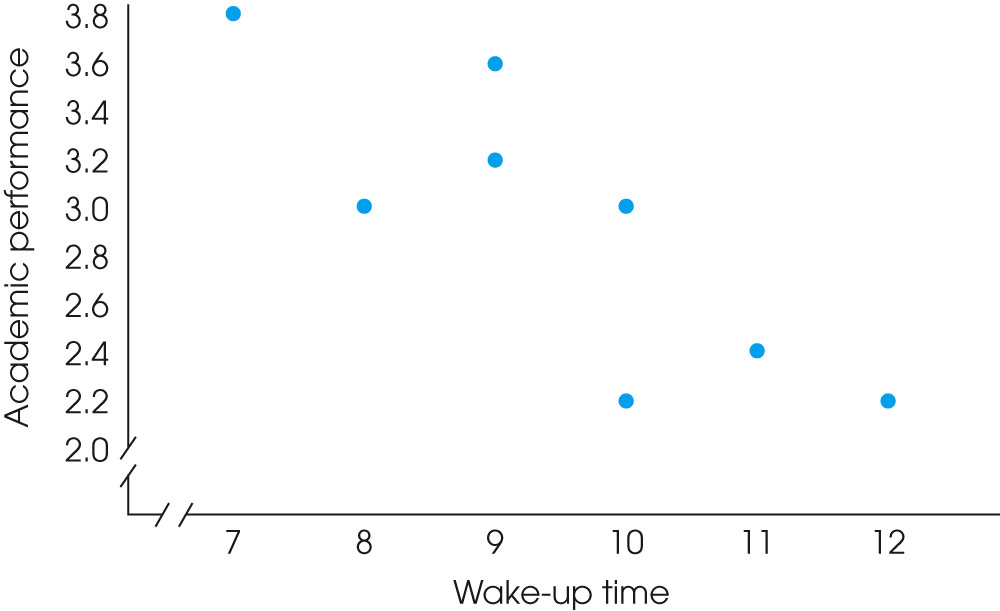
\includegraphics[width=0.45\textwidth]{FIGURES/wakeacademic2}}
      \only<2->{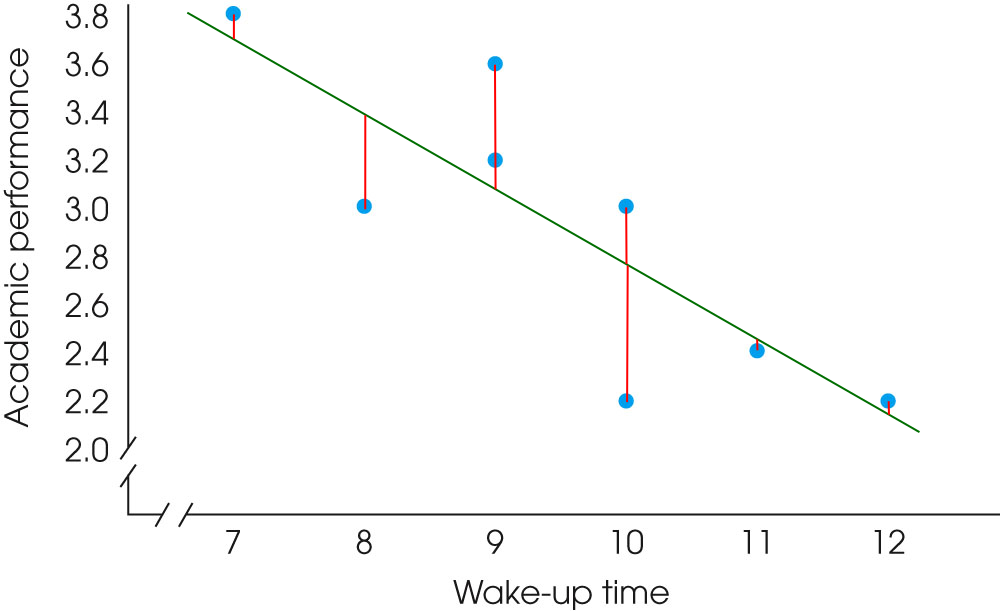
\includegraphics[width=0.45\textwidth]{FIGURES/wakeacademic3}}
    \end{tabular}
  \end{center}
  \begin{itemize}
  \item Wake-up time and academic performances measured for a sample of 8 children. Correlated?
    \pause
  \item It seems so, but the sample size is low!\pause
  \item And BTW, I got this data on the Net, no idea where it comes from, it could be fake!
  \end{itemize}
\end{frame}


\begin{frame}\frametitle{Linear Regression, Covariance, Correlation Coefficient}  
  $x = (x_1,\dots, x_N)$ wake-up-time variable, $y = (y_1,\dots,y_N)$ academic performance variable.
  \begin{itemize}
 \item Covariance between $x$ and $y$
    $$
    \cov(x,y) = \frac{1}{N}\sum_{i=1}^{N}\left(x_i-\bar{x}\right)\left(y_i - \bar{y}\right) = \frac{1}{N}\sum_{i=1}^Nx_iy_i - \bar{x}\bar{y}
    $$
  \item Linear regression: Find $a$ and $b$ such that 
    $$
    \sum_{i=1}^N|ax_i + b - y_i|^2 = \min: a = \frac{\cov(x,y)}{\sigma^2_x},\quad b \text{ is a bit too long}
    $$
    Here $a = -0.317$, $b = 5.933$. 
  \item How variations of one variable explains the other's: Pearson's correlation coefficient. 
    $$
    r = \frac{\cov(x,y)}{\sigma_x \sigma_y} = a\frac{\sigma_x}{\sigma_y}\in [-1,1]
    $$
    Here $r = -0.828$.
  \end{itemize}
\end{frame}

\begin{frame}\frametitle{Multivariate Data}
  Multivariate data $((x_1^1,x_2^1,\dots,x_p^1)^\top ,(x_1^N,x_2^N,\dots,x_p^N)^\top$ with $\bx^i=(x_1^i,x_2^i,\dots,x_p^i)^\top \in \RR^p$.
  \begin{columns}
    \begin{column}{0.5\textwidth}
      \begin{center}
        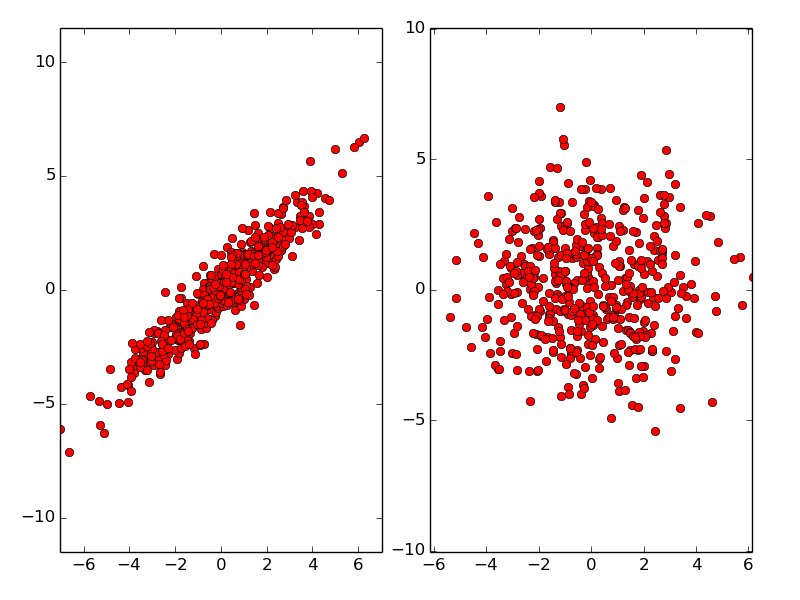
\includegraphics[width=1\textwidth]{FIGURES/bivariatesamespread}
      \end{center}
    \end{column}
    \begin{column}{0.5\textwidth}
      \begin{itemize}
      \item $p = 2$ here (else drawing complicated).
      \item Same spread along axes, but clear differences!
      \item Mean:
        $
        \bar{\bx} = \frac1N\sum_{i=1}^N \bx^i\in \RR^p. 
        $
      \item Covariance Matrix:
        $$
        \Sigma_\bx = \frac1N\sum_{i=1}^N\left(\bx_i-\bar{x}\right)\left(\bx_i-\bar{x}\right)^\top\in \RR^{p\times p}
        $$
      \end{itemize}
    \end{column}
  \end{columns}
  \begin{itemize}
  \item  In example from figure:
    $$
    \text{Left: } \Sigma_\bx = \begin{bmatrix}
      3.80  & 3.45\\
      3.45  & 3.61
    \end{bmatrix},\quad
    \text{right: } \Sigma_\bx = \begin{bmatrix}
      3.85  & 0.01\\
      0.01  & 4.27
    \end{bmatrix}
    $$
  \item In general: diagonal entry $(\Sigma_\bx)_{uu} = \sigma^2_{x_u}$, $(x_u = (x_u^1,\dots, x_u^N))$,
  \item off-diagonal entry $(\Sigma_\bx)_{uv} = \cov(x_u,x_v)$ 
  \end{itemize}
\end{frame}





\section{Random Variables}

\begin{frame}\frametitle{A Discrete Case: Casting A Dice}
  \begin{itemize}
  \item Here \myemph{random variable}: number returned after casting a dice $X$\vfill
  \item \myemph{Observed value}: $x$\vfill
  \item \myemph{State space}: Set of values of the random variable $S = \{1,2,3,4,5,6\}$.\vfill
  \item \myemph{Probability mass function}
    $$
    f(x) =
    \begin{cases}
      \frac16&x\in S\\
      0 & \text{else}.
    \end{cases}
    $$\vfill
  \item \myemph{Event}: subset of $S$.
  \end{itemize}
  \begin{center}
    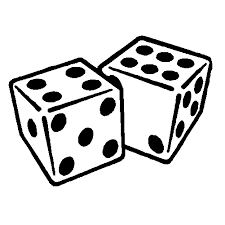
\includegraphics[width=0.2\textwidth]{FIGURES/castdice}
  \end{center}
\end{frame}


\begin{frame}\frametitle{Events and Probabilities}
  \begin{itemize}
  \item Event $E\subset S$.
  \item Examples:
    \begin{align*}
      &E_1 = \text{odd}: E_1 = \{1,3,5\}&\\
      &E_2 = \text{even}: E_2= \{2,4,6\}&\\
      &E_3 = X \leq 2: E_3 = \{1,2\}&
    \end{align*}
  \item Probability of an event:
    \begin{align*}
      &P(E_1) = \frac16 + \frac16 + \frac16 = \frac12&\\
      &P(E_2) = \frac16 + \frac16 + \frac16 = \frac12&\\
      &P(E_3) = \frac16 + \frac16 = \frac13&
    \end{align*}
  \item Dice casting: discrete random variable.
  \end{itemize}
\end{frame}



\begin{frame}\frametitle{A Continuous Case: Weight of a Strawberries Basket} 
 
  \tikz[overlay,remember picture]
  \node[anchor=south] at ($(current page.south)+(4,1.5)$) {
    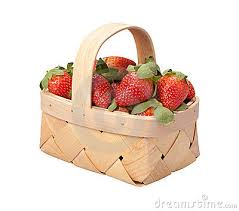
\includegraphics[width=0.7in]{FIGURES/strawberrybasket}
  };
  \begin{itemize}
  \item Random Variable: weight of a basket.
  \item Observed weight $x$
  \item Probability density function: $f(x)$.
  \item State space $S = [0,\infty[ $.
  \item \myemph{Probability density function}:
    $$
    f(x) \geq 0,\quad \int_0^\infty f(x)\,dx = 1.
    $$
  \item \myemph{Probability distribution}:
    $$
    P(X < t) = \int_0^t f(x)\,dx
    $$
  \end{itemize}
\end{frame}

\begin{frame}[t]{Weight of Strawberry Basket}
  \begin{itemize}
  \item Event $E_1$: weight $X < 400$g.  $P(E_1) = P(X < 400) = \int_0^{400} f(x)\,dx$. \vfill
  \item Event $E_2$: weight $X > 700$g.  $P(E_2) = P(X > 700) = \int_{400}^\infty f(x)\,dx$. \vfill
  \item $E_3$: $200\text{g} < X < 600$g. $P(E_3) =P(200\! <\! X\! <\! 600) \!=\! \int_{200}^{600}\!f(x)dx$
  \end{itemize}
\vfill
  \begin{center}
    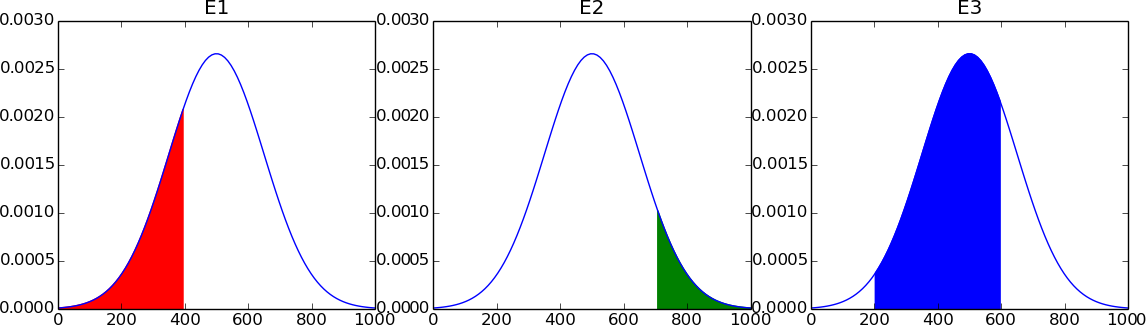
\includegraphics[width=0.99\textwidth]{FIGURES/contevents}
  \end{center}
\end{frame}


\begin{frame}[t]{Conditional Probabilities}

  \begin{itemize}
  \item An event probability may depend on another one!
  \item Probability that strawberry basket weight $<$ 500g in a supermarket depends on the probability that a customer ate one of them!
  \item Conditional Probability:
    $$
    P(E|F) = \frac{P(E\cap F)}{P(F)},\quad P(F)> 0.
    $$
    \pause
    \begin{itemize}[<+->]
    \item $P(E|F)$: Probability of $E$ \myemph{knowing} $F$.\vfill
    \item $P(E\cap F)$ common probability of $E$ and $F$, i.e., probability that $E$ and
      $F$ are realized simultaneously.\vfill
    \item Rewritten as Product Rule $P(E\cap F) =P(E|F) P(F)$
    \end{itemize}\pause
    \vfill
    \item Total Probability Theorem, important in classification! $(E_i)_i$ a pairwise complete disjoint set of events
      $
      E_i\cap E_j = \emptyset$, $i\not=j$, $\cup_i E_i = S$.
      Then 
      $$
      P(F) = P(F|E_1)P(E_1) + P(F|E_2)P(E_2) + \dots +  P(F|E_n)P(E_n)
      $$
  \end{itemize}
\end{frame}



\begin{frame}[t]{Dice Exercise}
  \begin{itemize}
  \item Two dice.
  \item Random Variables $X$: dice 1 value, and $Y$: dice 2 value.
  \item Events: 
    $$
    \begin{cases}
      E_1: & X = 1\\
      E_2: & X + Y = 4\\
      E_3: & Y = 4 
    \end{cases}
    $$
  \item Probabilities of Events:
    $$
    P(E_1) = \frac{1}{6},\quad P(E_2)= \frac3{36},\quad P(E_3) = \frac{1}{6}. 
    $$
  \item Combined Probabilities:
    $$
    P(E_1\cap E_2) =\frac1{36},\quad P(E_1\cap E_3) = \frac{1}{36}, \quad P(E_2\cap E_3) = 0.
    $$
  \end{itemize}
\end{frame}

\begin{frame}[t]{Dice Exercise}
  \begin{itemize}
  \item Cast the two dice. Dice 1 random variable is $Y$. \myemph{Observed}: Dice 1 ($X$) shows 1 $(X= 1)$.\\
    Probability that the sum of dice is 3, i.e. $X + Y = 3$ (event $E_2$).
    \vfill\pause
  \item Apply Conditional Probability Formula.\pause
    $$
    P(E_2|E_1) = \frac{P(E_1\cap E_2)}{P(E_1)} = \frac{\frac{1}{36}}{6} = \frac6{36} = \frac16
    $$
  \end{itemize}\vfill
\end{frame}


\begin{frame}[t]{Statistical Independence}
  \begin{itemize}
  \item Two events $E$ and $F$ are \myemph{independent} if the following equivalent conditions are satisfied
    $$
    P(E|F) = P(E) \Iff P(E\cap F) = P(E)P(F).
    $$
  \item Back to the Dice: We observe Dice 2: Probability for $Y= 4$ (event $E_3$):
    $$
    P(E_3|E_1) = \frac{\frac{1}{36}}{6} = \frac{1}{6} = P(E_3).
    $$
    Knowledge of event $E_1$ does not influence event $E_3$.
  \end{itemize}
\end{frame}


\begin{frame}[t]{Bayes Theorem}
  \begin{itemize}
  \item Many forms, very useful, many interpretations! \vfill
  \item Assume some statistical knowledge of event $E$ is given as $P(E)$. \vfill
  \item Then assume a new event $F$ is realized, we have $P(F|E)$. \vfill
  \item Bayes Theorem allows to update knowledge on $E$ as $P(E|F)$,
    $$
    P(E|F)=\frac{P(F|E)P(E)}{P(F)}
    $$
    \vfill
  \item $P(E)$ is called the \myemph{prior} (knowledge). \vfill
  \item $P(E|F)$ is called the \myemph{posterior}. \vfill
  \item $P(F|E)$ is called the \myemph{likelihood}. \vfill
  \item $P(F)$ is called the \myemph{evidence}.
  \item Proof is straightforward.
    $$
    P(E|F) := \frac{P(E\cap F)}{P(F)} = \frac{P(E\cap F)}{P(E)}\frac{P(E)}{P(F)} = \frac{P(F|E)P(E)}{P(F)}
    $$
  \end{itemize}
\end{frame}

\begin{frame}[t]{Strawberries Again}
  \begin{itemize}
  \item Events.
    \begin{itemize}
    \item Event $E$: someone ate some of my strawberries.
    \item Event $F$: $X < 450$.g
    \end{itemize}
  \item Prior knowledge.
    \begin{itemize}
    \item $P($someone ate some of my strawberries$) = 0.75$ (I am suspicious by nature).
    \item $P($no one ate my strawberries$) = 0.25)$.
    \end{itemize}
  \end{itemize}
  \begin{center}
    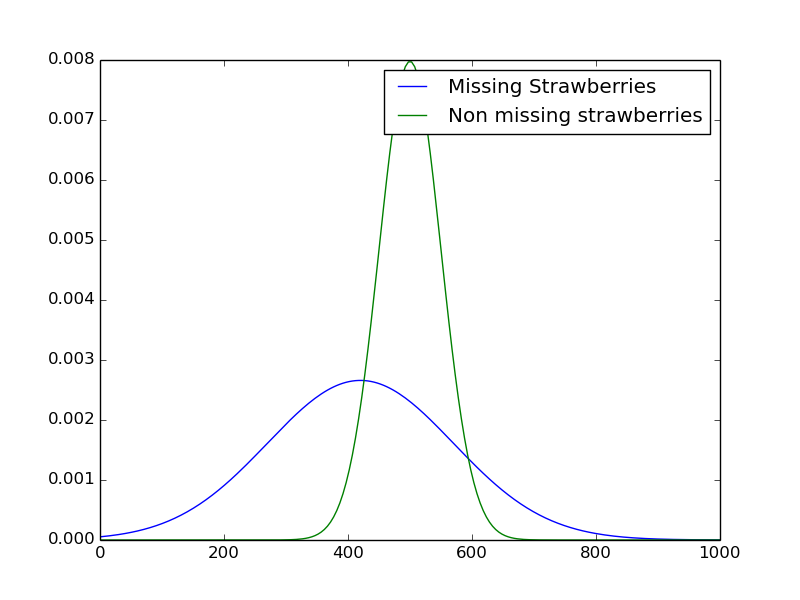
\includegraphics[width=0.6\textwidth]{FIGURES/strawberryweightdistribs}  
  \end{center}
\end{frame}



\begin{frame}[t]
  \begin{itemize}
  \item I have a basket with less than 450g strawberries.
    \begin{align*}
    &P(X < 450 | \text{ missing}) = 0.58&\\
    &P(X < 450 | \text{ not missing}) = 0.16\,\, (\text{risky business)}&
  \end{align*}
\end{itemize}
\begin{center}
  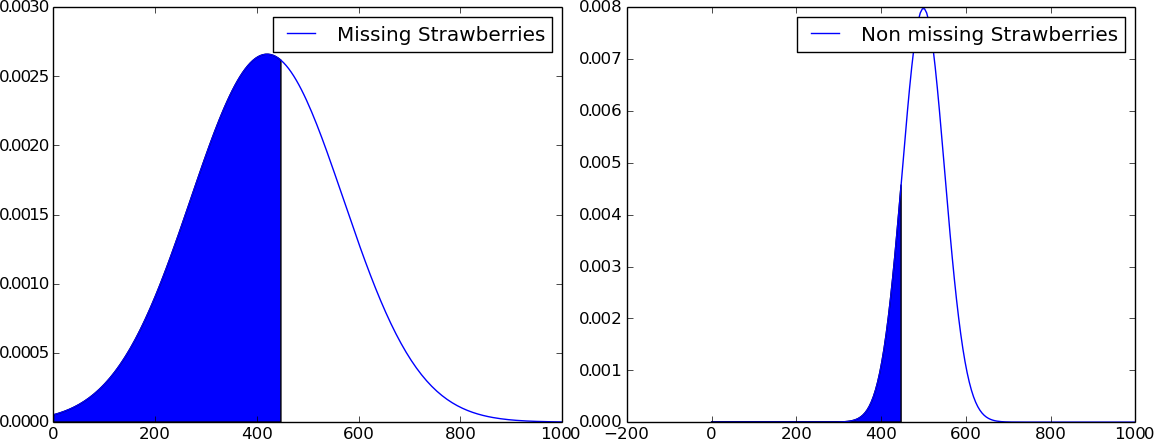
\includegraphics[width=0.8\textwidth]{FIGURES/strawberriesmissing}
\end{center}
\begin{itemize}
\item Update our knowledge thanks to Bayes:
  \begin{align*}
    P(\text{eaten } | X < 450 ) &
    =\frac{P(X < 450 | \text{ eaten}) P(\text{eaten})}{P(X < 450)}\\
    &=\frac{0.58*0.75}{0.58*0.75 + 0.16*0.25} = 0.92
  \end{align*}
\end{itemize}
\end{frame}




\begin{frame}[t]{Moments of a Discrete Random Variable}
  \begin{itemize}
  \item Discrete variable $X$, state space $\{x_1, x_2, \dots
    x_k\}\subset \RR$ with probability mass $P(X)$: $P(x_i) = p_1$
    with $p_1 + p_2 + \dots p_k = 1$, $p_i >= 0$.
  \item Expectation of $X$:
    $$
    E(X) = x_1p_1 + x_2p_2 + \dots x_k p_k = \sum_{i=1}^k x_i p_i = \sum_{i=1}^kx_i P(x_i)
    $$
  \item In general, if $F:\RR\to \RR$ a function which transform the value of $X$, $F(X)$ new random variable with expectation
    $$
    E(F(X)) = \sum_{i=1}^k f(x_i)p_i
    $$
  \item Variance of $X$:
    $$
    \sigma_X = \sum_{i=1}{\left(n_i - E(X)\right)^2p_i} = E\left(\left(X-E(X)\right)^2\right) = E(X^2) - E(X)^2
    $$
  \item Order $n$ moments, non centered and centered:
    $$
    E(X^n) = \sum_{i=1}^n x_i^n p_i,\quad E\left(X-E(X)\right)^n = \sum_{i=1}^n\left(x_i- E(X)\right)^np_i
    $$
  \end{itemize}
\end{frame}




\begin{frame}[t]{Moments of a Continuous Random Variable}
  \begin{itemize}
  \item Continuous variable $X$, state space $S=\RR$ with probability density function $p(x)$,
    $$
    \int_{-\infty}^\infty p(x)\,dx = 1.
    $$
  \item Expectation of $X$:
    $$
    E(X) = \int_{-\infty}^\infty x \,p(x)\,dx
    $$
  \item In general, if $F:\RR\to \RR$ a function which transform the value of $X$, $F(X)$ new random variable with expectation
    $$
    E(F(X)) = \int_{-\infty}^\infty F(x) \,p(x)\,dx
    $$
  \item Variance of $X$:
    $$
    \sigma_X = \int_{-\infty}^\infty \left(x - E(x)\right)^2 \,p(x)\,dx = E\left(X-E(X)\right)^2 = E(X^2) - E(X)^2.
    $$
  \item Order $n$ moments, non centered and centered:
    $$
    E(X^n) = \int_{-\infty}^\infty x^n\,dx,
    \quad E\left(X-E(X)\right)^n =
    \int_{-\infty}^{\infty}\left(x - E(x)\right)^n\,dx.
    $$
  \end{itemize}
\end{frame}


\begin{frame}[t]{Discrete Vector Valued Random Variable}
  \begin{itemize}
  \item item ${\bX = (X,Y)^\top}$ position on a grid. State space: a finite subset of $\RR^n$, probability mass $P(X,Y)$ with
    $$
    p(x_i,y_i) \geq 0,\quad \sum_{i=1}^n{p(x_i,y_i)} = 1. 
    $$
  \item \myemph{Expectation Vector}: $E(\bX)$: component-wise expectation/average
    $$
    E(\bX) = E((X,Y)^\top) = \sum_{i=1}^n
    \begin{bmatrix}
      x_i\\y_i
    \end{bmatrix}
    p(x_i,y_i) =
    \begin{bmatrix}
      \sum_{i=1}^n x_i p(x_i,y_i)\\
      \sum_{i=1}^n y_i p(x_i,y_i)
    \end{bmatrix}
    =
    \begin{bmatrix}
      E(X)\\
      E(Y)
    \end{bmatrix}
    $$
  \item \myemph{Covariance Matrix} $\Sigma_\bX$
    \begin{align*}
      &\Sigma_\bX \!=\! \sum_{i=1}^n\udesc{\text{outer product}}
      {
        \left(
          \begin{bmatrix}
            x_i\\y_i
          \end{bmatrix}
          \!-E(\bX)
        \right)\!
        \left(
          \begin{bmatrix}
            x_i\!&y_i
          \end{bmatrix}
          \!-E(\bX)^\top
        \right)
      }
      = \sum_{i=1}^n
      \begin{bmatrix}
        x_i-E(X)\\y_i-E(Y)
      \end{bmatrix}
      \begin{bmatrix}
        x_i-E(X) & y_i-E(Y)
      \end{bmatrix}&\\
      &=\sum_{i=1}^n
      \begin{bmatrix}
        \left(x_i-E(X)\right)^2 & \left(x_i-E(X)\right)\left(y_i-E(Y)\right)\\
        \left(x_i-E(X)\right)\left(y_i-E(Y)\right) &  \left(y_i-E(Y)\right)^2 
      \end{bmatrix}&
    \end{align*}
  \end{itemize}
  
\end{frame}

\begin{frame}[t]{Continuous Vector-valued Random Variables}
  \tikz[overlay,remember picture]
  \node[anchor=north] at ($(current page.north)+(4,-3)$) {
    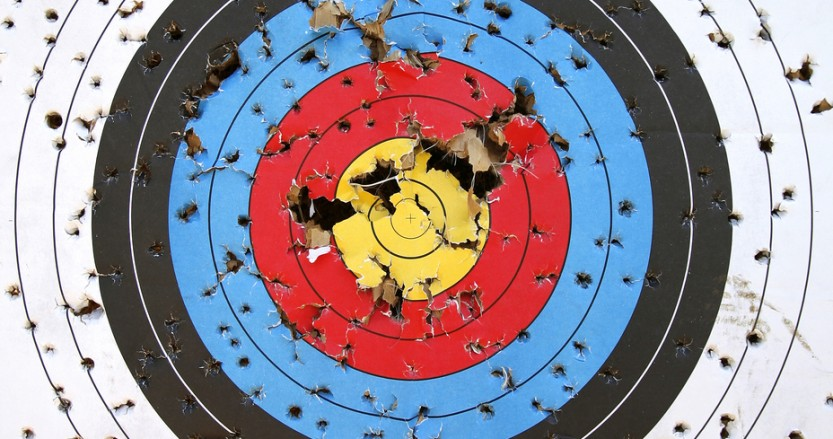
\includegraphics[width=1in]{FIGURES/shotgunorriffle}
  };
  \begin{itemize}
  \item ${\bX = (X,Y)^\top}$ position of a bullet/dart on a target
    $(x,y)^\top$. State space $S = \RR^2$ (well...). Probability density
    function $p(x,y) \geq 0$,
    $$
    \int_{-\infty}^{\infty}\int_{-\infty}^{\infty}p(x,y)\,dx,dy = 1.
    $$
  \item Probability distribution 
    $$
    P(X< s, Y < t) = \int_{-\infty}^s\int_{-\infty}^t f(x,y)\,dx\,dy.
    $$
  \item Expectation \myemph{vector}
    $$
    E(\bX) =  \left(E(X),E(Y)\right)^\top = \int_{-\infty}^{\infty}\int_{-\infty}^{\infty}(x,y)^\top p(x,y)\,dxdy
    $$  
  \end{itemize}
  \begin{center}
    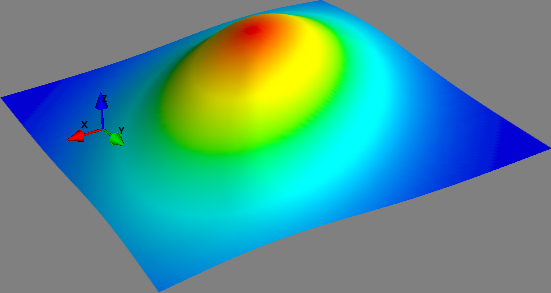
\includegraphics[width=0.3\textwidth]{FIGURES/bivariateGauss}
  \end{center}
\end{frame}


\section{A Few Laws}


\begin{frame}[t]{Bernoulli Distribution}
  \begin{itemize}
  \item A simple random variable $X$ with two states: $S = \{0,1\}$
  \item Probability mass function $P((X=0) = p \in ]0,1[$, $P(X=1) = 1-p$.
  \item $p$ is the \myemph{parameter} of the distribution.
  \item Expectation:
    $$
    E(X) = 0.p + 1.(1-p) = 1-p
    $$
  \item Variance:
    $$
    \sigma^2_X = E(X-(1-p))^2 = (0-(1-p))^2.p + (1-p - (1-p))^2.(1-p) = p(1-p)^2
    $$
  \item Spread/standard deviation = $\sqrt{\text{variance}}$:
    $$
    \sigma_X = (1-p)\sqrt{p}
    $$
  \end{itemize}
\end{frame}




\begin{frame}[t]{Binomial Distribution}
  \begin{itemize}
  \item Number of success (1) in $n$ repeated Bernoulli experiment.
  \item $X_1,\dots,X_n$ random variables each with Bernoulli distribution with same parameter $p$.
  \item Binomial distribution with parameters $(p,n)$: $X = X_1+ X_2\dots+X_n$. State space: $S = \{0,1,\dots, n\}$.
  \item Probability mass?
    \begin{center}
      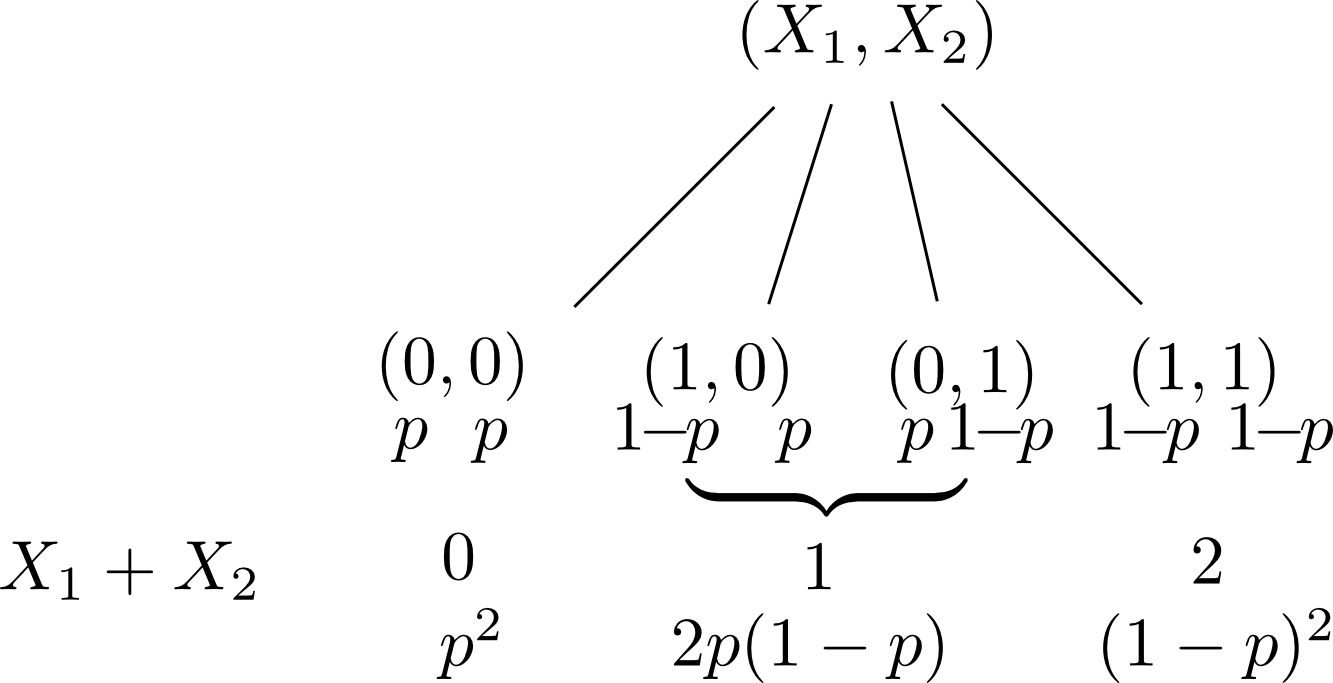
\includegraphics[width=0.5\textwidth]{FIGURES/binomial2.png}
    \end{center}
    $$
    P(X = 0) = p^2,\quad P(X=1) = 2p(1-p),\quad P(X=2) = (1-p)^2.
    $$
    \item Binomial formula for $n=2$: $1 = 1^2 = (p + (1-p))^2 = p^2 + 2p(1-p) + (1-p)^2$!
    \item Expectation, variance?
  \end{itemize}
\end{frame}



\begin{frame}[t]{Binomial Law: Excercise}
  \begin{itemize}
  \item $n=3$, $X = X_1+X_2+X_3$. How many possible cases for values of triple $(X_1,X_2,X_3)$
  \item Probability mass for $X$
  \item Moments (expectation, variance...).
  \end{itemize}
  \begin{center}
    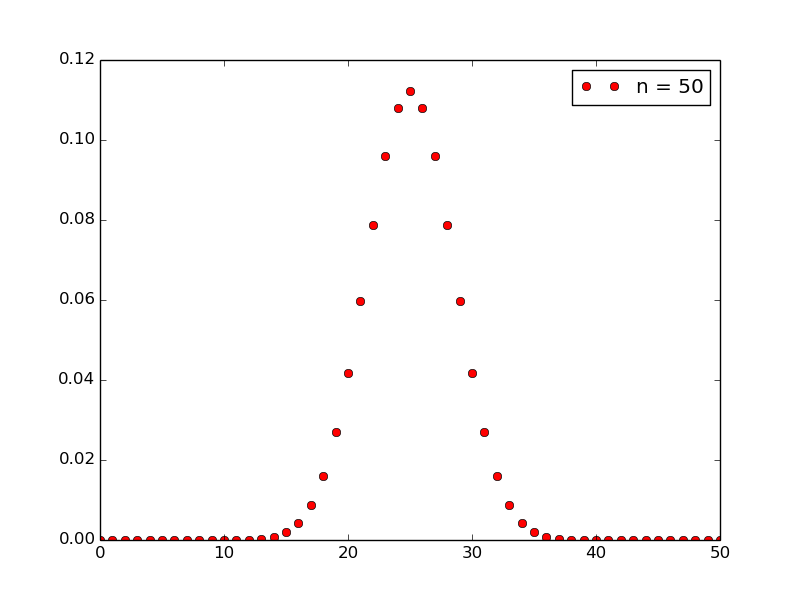
\includegraphics[width=0.7\textwidth]{FIGURES/binomial50}
  \end{center}
\end{frame}


\begin{frame}[t]{Uniform Distribution on a Segment}
  \begin{itemize}
  \item Continuous. State space $S = [a,b]\in\RR$. $X$ random variable: all values are \myemph{equiprobable}.
  \item Probability density function
    $$
    p(x) = \frac{1}{b-a},\quad\text{independent of }x!: \int_a^b\frac{dx}{b-a} = 1
    $$
  \item Expectation:
    $$
    E(X) = \int_a^b\frac{x}{b-a} \,dx = \frac{a+b}{2}
    $$
    Average position is the mid-point!
  \item Variance:
    $$
    \sigma_X^2 =  \frac{1}{b-a}\int_a^b  \left(x-\frac{a+b}{2}\right)^2\,dx = \frac{(b-a)^2}{12}
    $$
  \end{itemize}
\end{frame}


\begin{frame}[t]{1D Gaussian}
  \begin{itemize}
  \item Continuous Random Variable $X$. Maybe the most important one, due to the celebrated Central Limit Theorem.
  \item State space $\RR$.
  \item Parameters: $\mu\in \RR$, $\sigma\in ]0,\infty[$.
  \item Probability density function 
    $$
    p_{\mu,\sigma}(x) = \frac{1}{\sqrt{2\pi\sigma^2}}e^{-\frac{(x-\mu)^2}{2\sigma^2}}
    $$
  \item Classical theorem shows that
    $$
    \int_{-\infty}^\infty  p_{\mu,\sigma}(x)\,dx = 1.
    $$
  \item Expectation: $E(X) = \mu$.
  \item Variance $\sigma_X^2 = \sigma$.
  \item Continuous limiting case for normalized binomial distribution when $n\to\infty$. 
  \end{itemize}
\end{frame}



\begin{frame}
  \begin{center}
    {   \Huge The End}
    ~\\
    ~\\
{\large Please read Forsyth and Ponce chapter on probabilities.}
  \end{center}
\end{frame}




% \section{Probabilities Abstract Nonsense}
% \label{sec:proban}

% \begin{frame}
%   \frametitle{Universe, Outcomes, Events}
%   \begin{columns}
%     \begin{column}{0.6\textwidth}
%       \begin{itemize}[<+->]
%       \item \myemph{Universe} $\Omega$: each element corresponds to an ``outcome'', a
%         ``state'' \dots Should describe all possible states / outcomes of a system.
%       \item \myemph{Tribe} or \myemph{$\sigma$-algebra} $\Ff$: set of subsets of $\Omega$
%         with specific properties.
%       \item \myemph{Event}: element of a given tribe, thus, subset of $\Omega$.
%       \item \myemph{Probability} on $\Ff$: A function $P$ defined on elements of $\Ff$,
%         i.e., specific subsets of $\Omega$: $P:A\subset\Omega\mapsto P(A)\in[0,1]$, with
%         \begin{align*}
%           &P(\emptyset)=0,\quad P(\Omega)=1,&\\ 
%           &P(A\cup B) = P(A) + P(B) \text{ if } A\cap B=\emptyset&          
%         \end{align*}
%       \end{itemize}
%     \end{column}\pause
%     \begin{column}{0.4\textwidth}
%       \begin{center}
%         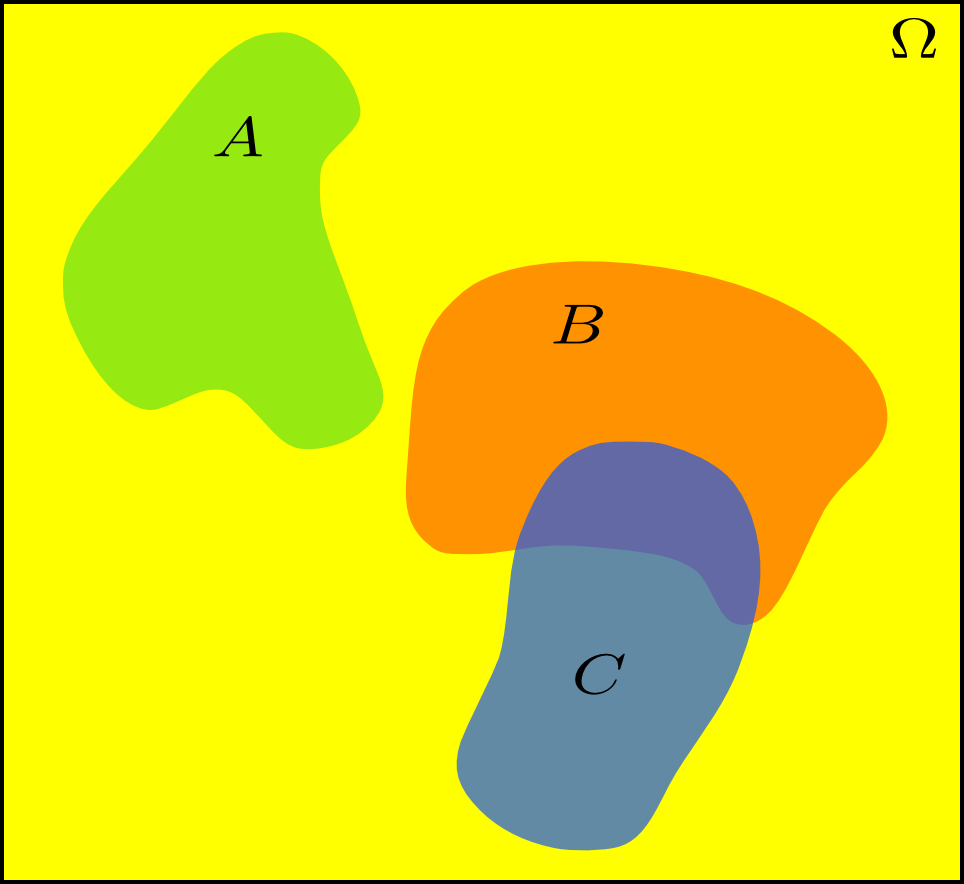
\includegraphics[width=0.9\textwidth]{FIGURES/universe}
%       \end{center}
%       $\Omega$ ``square of length 1'', $P(A) = $ area of $A\subset \Omega$.
%     \end{column}
%   \end{columns}\pause
%   In general $\Ff$ is chosen ``as large as possible, but not too large'': subject of Measure Theory in Mathematics.
% \end{frame}


% \begin{frame}\frametitle{Examples}
%   \begin{columns}
%     \begin{column}{0.6\textwidth}
%       \begin{itemize}[<+->]
%       \item Coins: Two configurations: head and tail $\Omega = \mathtt{h,t}$.
%       \item Tribe: $\Ff_1 = \{\emptyset, \{\mathtt{h,t}\}\}$ or 
%         $\Ff_2 = \{
%         \emptyset, \{ \mathtt{h} \}, \{ \mathtt{t} \}, \{ \mathtt{h,t}\}
%         \}$ (better)
%       \item Probability for $\Ff_2$: $P(\emptyset)=0$, $P(\Omega) = 1$.
%         $P(\{\mathtt{h}\}) = p\in [0,1]$, $P(\{\mathtt{t}\}) = 1-p$.\\
%         In general, $p= 0.5$ or someone is cheating\dots
%       \end{itemize} 
%     \end{column}
%     \begin{column}{0.4\textwidth}
%       \begin{center}
%         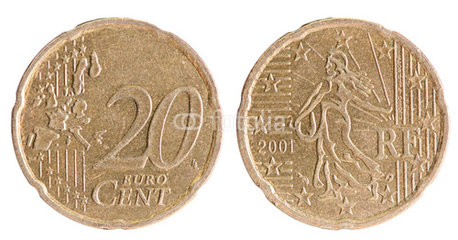
\includegraphics[width=0.7\textwidth]{FIGURES/Euro2cents}
%       \end{center}
%     \end{column}
%   \end{columns}\pause
%   \begin{columns}
%     \begin{column}{0.6\textwidth}
%       \begin{itemize}[<+->]
%       \item Dice: 6 configurations $\Omega = \{1,2,3,4,5,6\}$. 
%       \item Tribe: the largest one $\Ff$ contains all the possible subsets of $\Omega$. How many?
%       \item Probability? $P(\{i\}) = p_i\in [0,1]$ with $p_1 + p_2 + p_3 + p_4 + p_5 + p_6 = 1$.
%       \item In most cases, $p_1 = p_2 = p_3 = p_4 = p_5 = p_6 = 1/6$.
%       \end{itemize}
%     \end{column}
%     \begin{column}{0.4\textwidth}
%       \begin{center}
%         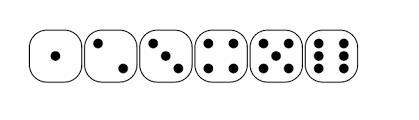
\includegraphics[width=0.8\textwidth]{FIGURES/dice}
%       \end{center}
%     \end{column}
%   \end{columns}
% \end{frame}




% \begin{frame}\frametitle{Conditional Probabilities, Independence, Bayes' Theorem}
%   \begin{columns}
%     \begin{column}{0.4\textwidth}
%       \begin{center}
%         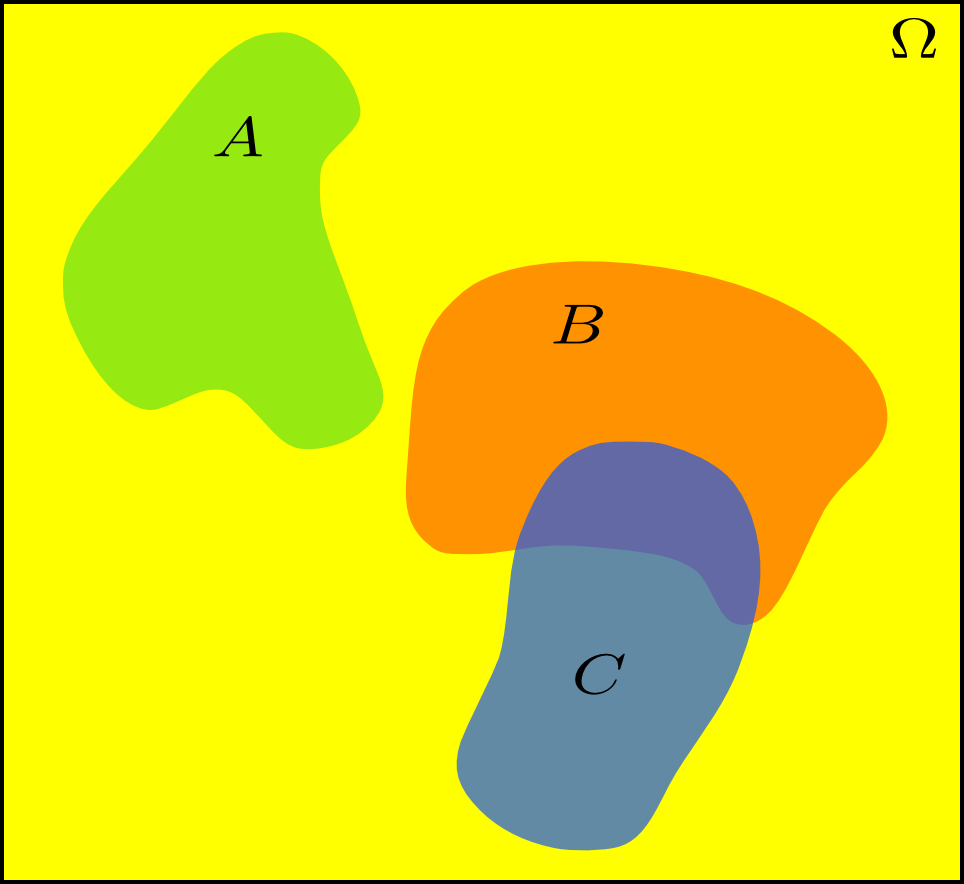
\includegraphics[width=0.9\textwidth]{FIGURES/universe}
%       \end{center}
%     \end{column}
%     \begin{column}{0.6\textwidth}
%       \begin{itemize}
%       \item $P(A|B)$: Probability of event $A$ knowing that event $B$ is realized.
%         $$
%         P(A|B) = \frac{P(A\cap B)}{P(B)}
%         $$
%       \item Independence of events $A$ and $B$ are independent if $P(A|B) = P(A)$: the
%         knowledge of $B$ does not influence the realization (or not) of $A$.\\
%       \item Equivalently: $A$ and $B$ independent iff
%         $$
%         P(A\cap B) = P(A) P(B).
%         $$
%       \end{itemize}
%     \end{column}
%   \end{columns}
%   \begin{itemize}
%   \item Bayes' Theorem, Retrodiction Rule, Probability of Causes...
%     $$
%     P(B|A) = \frac{P(A|B)P(B)}{P(A)}
%     $$
%     Proof: Write en compare $P(A|B)$ and $P(B|A)$! ($A\cap B = B\cap A$)
%   \end{itemize}
% \end{frame}

\end{document}


